% dfa-re-kleene.tex

\documentclass[tikz]{standalone}
\usetikzlibrary{positioning, decorations.pathmorphing}

\begin{document}
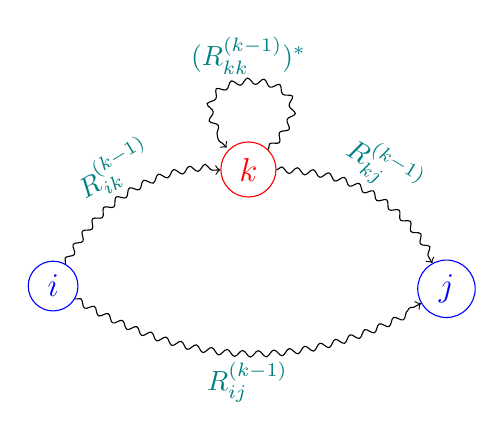
\begin{tikzpicture}[v/.style = {draw, circle, minimum size = 8pt, font = \large},
    every edge/.style = {draw, ->},
    path/.style = {->, decorate, decoration = {snake, amplitude = .4mm, segment length = 2mm, post length = 1mm}}]
  \node (i) [v, blue] {$i$};
  \node (k) [v, red, above right = 1.0cm and 2.0cm of i] {$k$};
  \node (j) [v, blue, below right = 1.0cm and 2.0cm of k] {$j$};

  \path (i) edge[path, bend right] node [teal, below] {$R_{ij}^{(k-1)}$} (j)
	(i) edge[path, bend left] node [teal, above, sloped] {$R_{ik}^{(k-1)}$} (k)
	(k) edge[path, loop] node [teal, above, sloped] {$(R_{kk}^{(k-1)})^{\ast}$} (k)
	(k) edge[path, bend left] node [teal, above, sloped] {$R_{kj}^{(k-1)}$} (j);
\end{tikzpicture}
\end{document}